%%%%%%%%%%%%%%%%%%%%%%%%%%%%%%%%%%%%%%%%%
% Szablon pracy dyplomowej
% Wydział Informatyki
% Zachodniopomorski Uniwersytet Technologiczny w Szczecinie
% autor Joanna Kołodziejczyk (jkolodziejczyk@zut.edu.pl)
% Bardzo wczesnym pierwowzorem szablonu był
% The Legrand Orange Book
% Version 2.1 (26/09/2018)
%
% Modifications to LOB assigned by %JK
%%%%%%%%%%%%%%%%%%%%%%%%%%%%%%%%%%%%%%%%%

%----------------------------------------------------------------------------------------
%	CHAPTER 1
% 	author: Joanna Kolodziejczyk (jkolodziejczyk@zut.edu.pl)
%----------------------------------------------------------------------------------------

\chapter{Wprowadzenie teoretyczne}\label{ch:wprowadzenie-teoretyczne}
\chaptermark{Wprowadzenie teoretyczne}

Na przestrzeni ostatnich lat stosowanie Systemów Automatycznego Rozpoznawania Tablic Rejestracyjnych (ARTR) (ang. \textit{Automatic Licence Plate Recognition} --- ALPR) stało się znacznie bardziej powszechne.
W większości dużych miast istnieją parkingi, gdzie po umieszczeniu opłaty za postój, przy zbliżeniu się do wyjazdu, szlaban otwiera się automatycznie po rozpoznaniu numeru rejestracyjnego pojazdu, w którym się poruszamy.
W obecnych czasach wszystkie nowoczesne systemy do zarządzania i sterowania ruchem drogowym oparte są o technologie ARTR.
Instytucje takie jak służby drogowe, dzięki rejestrowanym i przetwarzanym w czasie rzeczywistym ogromnym ilościom danych, są \\w stanie odpowiednio szybko reagować na wydarzenia na drogach takie jak kolizje, korki lub innego rodzaju utrudnienia.
Innym z możliwych przykładów zastosowania wspomnianych systemów są odcinkowe pomiary prędkości, opłaty za przejazd płatnymi drogami lub wykrywanie kierowców łamiących przepisy.
Dzięki nieustannemu rozwojowi technologii i co raz wydajniejszym komputerom, systemy stają się tańszą i łatwiej dostępną alternatywą dla systemów opartych na RFID (ang. \textit{Radio-frequency identification}), które to wymagają specjalnej etykiety do prawidłowego działania.

Rozpoznawanie tablic rejestracyjnych jest techniką polegająca na wykryciu i odczytaniu znaków z tablicy rejestracyjnych na podstawie zarejestrowanego obrazu.
Do tego celu wykorzystywany jest aparat o wysokiej rozdzielczości oraz odpowiedni program komputerowy.
Oprogramowanie otrzymuje na wejściu cyfrową reprezentację obrazu.
Dla zdjęć kolorowych każdy piksel opisany jest wartościami z palety barw RGB reprezentującymi jego barwę oraz współrzędnymi umiejscowienia w obrazie.
Dla zdjęć monochromatycznych barwy opisywane są najczęściej za pomocą wartości luminacji obrazu.

W procesie automatycznego rozpoznawania tablic rejestracyjnych pozyskany obraz jest odpowiednio przetwarzany.
Przed przejściem do rozpoznawania, obraz często jest konwertowany do skali szarości i filtrowany za pomocą filtrów np.
(Gaussa lub średnio-przepustowego) w celu redukcji szumu.
W procesie tym można wyróżnić trzy etapy~\cite{1688109}:
\begin{itemize}
    \item \textbf{detekcję} - określenie położenia tablicy rejestracyjnej w analizowanym obrazie
    \item \textbf{segmentację} - wyodrębnienie pojedynczych znaków na fragmencie obrazu ze zlokalizowaną tablicą
    \item \textbf{identyfikację} - rozpoznanie każdego ze znaków i przedstawienie ich w formie tekstowej, którą można później wykorzystać do dalszych działań w zależności od przeznaczenia systemu
\end{itemize}
\FloatBarrier
Na Rysunku~\ref{fig:schemat_lpr} przedstawiono graficzną reprezentację powyższego procesu.
\begin{figure}[!ht]
    \centering
    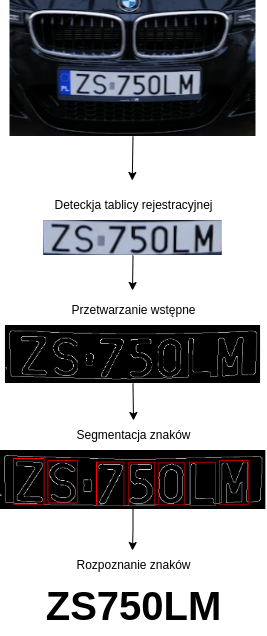
\includegraphics[scale=0.6]{Pictures/schemat_lpr}
    \caption{Etapy procesu automatycznego rozpoznawania tablic rejestracyjnych (źródło: opracowanie własne).}
    \label{fig:schemat_lpr}
\end{figure}
\FloatBarrier
Kolejne etapy korzystają z wyników uzyskanych w poprzednich krokach, co oznacza, że błąd powstały we wcześniejszej fazie, będzie rzutował na jakość działania całego systemu.
W wielu systemach zanim dojdzie do rozpoznawania tablicy rejestracyjnej, obraz jest wpierw odpowiednio przetwarzany.
Jednymi z najpowszechniej stosowanych czynności są skalowanie obrazu, modyfikacje jasności oraz redukcja zakłóceń.
W zależności od wymagań stawianych przed danym mechanizmem i środowiskiem jego działania, czynności te mogą znacznie się od siebie różnić.
Najbardziej podstawowe systemy wymagają, aby pojazd znajdował się nieruchomo w określonym miejscu.
Tego typu rozwiązania najczęściej stosowane są na parkingach, gdzie szlaban otwiera się po odczycie numerów rejestracyjnych pojazdu i potwierdzeniu opłaty za postój w zewnętrznej bazie danych.
Takie systemy pracują z reguły w środowisku o niskim poziomie zakłóceń wynikających z warunków atmosferycznych i oświetlenia.
Obecnie na rynku znajduje się wiele komercyjnych rozwiązań, które oferują wysoką dokładność (powyżej 95\%) dla tego rodzaju detekcji.
Taki rodzaj systemów ARTR nazywany systemami statycznymi.
Dużo większą złożonością charakteryzują się systemy dynamiczne, w których znacznie większą rolę odgrywają zakłócenia wynikające ze zmiennych warunków oświetlenia.
W obecnych czasach stworzenie dynamicznego systemu ARTR o wysokiej dokładności wciąż stanowi wyzwanie i jest tematem wielu prac naukowych.
Celem niniejszej pracy jest analizowanie obrazów pochodzących z kamery samochodowej, co zdecydowanie sprawia, że jest to system dynamiczny.
Poniżej przedstawiono najczęściej stosowane metody widzenia komputerowego w systemach ARTR\@.


\section{Przegląd istniejących metod detekcji tablic rejestracyjnych}
\index{Przegląd istniejących metod detekcji tablic rejestracyjnych}

Zgodnie ze słowikiem języka polskiego, definicja tablicy rejestracyjnej brzmi następująco:
\begin{definition}[Tablica rejestracyjna]
    Płytka zawierająca numery identyfikacyjne pojazdu, umieszczana z przodu i z tyłu pojazdu.
\end{definition}
Dla programu komputerowego powyższe zdanie jest niezrozumiałe.
W zadaniu detekcji tablicy rejestracyjnej, wymagane jest, aby maszyna ``zrozumiała'' jakich obiektów należy szukać.
W tym kontekście, za definicję można uznać ``prostokątny obszar, z dużym zagęszczeniem horyzontalnych i wertykalnych krawędzi''\cite{824138}.
W oparciu o powyższe cechy zaprezentowano wiele algorytmów do rozwiązania zadania wykrywania tablic rejestracyjnych.
Część z nich wywodzi się z tradycyjnych metod widzenia komputerowego i metod głębokiego uczenia.
Każda z metod ma swoje zalety, ale również często ograniczenia.
W związku z tym, trudno jednoznacznie stwierdzić, która z metod jest najbardziej efektywna.

Detekcja numerów rejestracyjnych jest wyzywającym zadaniem ze względu na poniższe czynniki:
\begin{itemize}
    \item tablica rejestracyjna zajmuje niewielki obszar na zdjęciu
    \item istnienie ogromnej ilości formatów tablic rejestracyjnych (w zależności od kraju rejestracji lub rodzaju pojazdu)
    \item słabe oświetlenie, rozmazany obraz, refleksy świetlne
    \item ruch pojazdu, zabrudzone tablice
\end{itemize}
Tradycyjne metody widzenia komputerowego oparte są na cechach takich jak kształt, kolor, symetria, tekstury itp.\cite{9310202}.
W celu uzyskania lepszych wyników, spotyka się rozwiązania, w których łączy się wiele technik.
Poniżej wyróżniono najczęściej stosowane metody w detekcji tablic rejestracyjnych.

\subsection{Metody oparte na krawędziach (ang. \textit{edge based)}}
Biorąc pod uwagę, że tablica rejestracyjna jest prostokątem o znanych proporcjach, większość badań bazuje na podejściu opartym o wykrywanie krawędzi.
W większości przypadków kolor tablicy rejestracyjnej jest różny od koloru pojazdu.
Dzięki temu, granice tablicy zostają uznane za krawędzie.
Wiele metod wykorzystuje filtr Sobela.
Jego działania polega dyskretnym różniczkowaniu i aproksymacji pochodnych kierunkowych intensywności obrazu.
Filtr ten składa się z dwóch macierzy o wymiarach 3x3 (\ref{fig:sobel_filter}) służących do detekcji krawędzi horyzontalnych i wertykalnych.
\FloatBarrier
\begin{figure}[!ht]
    \centering
    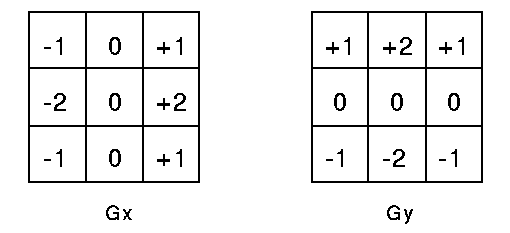
\includegraphics[scale=0.6]{Pictures/sobel_filter}
    \caption{Macierze detektora krawędzi Sobela (źródło: opracowanie własne).}
    \label{fig:sobel_filter}
\end{figure}
\FloatBarrier
Zaletą takiego podejścia jest niewątpliwa łatwość użycia, natomiast jedną z głównych wad jest jego wrażliwość na szum.

Często wykorzystywaną metodą do wykrywania krawędzi obiektów w obrazach jest \textit{Binary Image Processing}.
Technika ta polega na sprowadzenia obrazu do postaci, w której kolory pikseli przyjmują tylko dwie wartości - czarną lub białą.
Osiąga się to za pomocą ustalenia progu, który determinuje kolor piksela.
Próg wyznaczany jest na podstawie histogramu obrazu w odcieniach szarości.
Metoda ta jest użyteczna, ze względu na fakt łatwego odseparowania obiektu od tła.
Wykorzystuje ona założenie, że krawędzie tablicy są proste i poziome.
Przy zdeformowanych lub zabrudzonych tablicach, algorytm ten nie osiąga zadowalających wyników.

Inną stosowaną metodą do wykrywania linii na obrazach binarnych jest transformata Hougha~\cite{DuanBuildingAA}.
Motywacją do jej opracowania była metoda siłowa (ang. \textit{brute force}), która jest jednak znacznie bardziej zasobożerna.
Złożoność algorytmu siłowego wynosi $O(n^3)$.
Transformata Hougha polega na twierdzeniu, że każda prosta może być jednoznacznie przedstawiona za pomocą dwóch parametrów.
Przestrzeń tych parametrów to właśnie przestrzeń Hougha.
Najczęściej używanymi parametrami są współczynniki $\rho$ i $\alpha$ z równania prostej w postaci normalnej~\eqref{eqn:transform_hough}.
\begin{equation}
    \label{eqn:transform_hough}
    x\cos{\alpha} + y\sin{\alpha} = \rho
\end{equation}
W powyższym równaniu $\rho$ jest promieniem wodzącym, natomiast $\alpha$ kątem tworzonym przez $\rho$ z osią X.
W związku z powyższym, jest to algorytm o liniowej złożoności obliczeniowej.
Można wykazać następujące własności transformacji Hougha:\\
\begin{theorem}
    Prostej przestrzeni kartezjańskiej odpowiada w przestrzeni Hougha punkt, natomiast
    punktowi przestrzeni kartezjańskiej odpowiada w przestrzeni Hougha sinusoidalna krzywa.
    Punkty leżące na tej samej prostej korespondują z sinusoidami przechodzącymi przez
    wspólny punkt w przestrzeni Hougha~\cite{hough_transform_definition}.
\end{theorem}
Zasadę transformacji ilustruje Rysunek~\ref{fig:hough_transform}.
\begin{figure}[!ht]
    \centering
    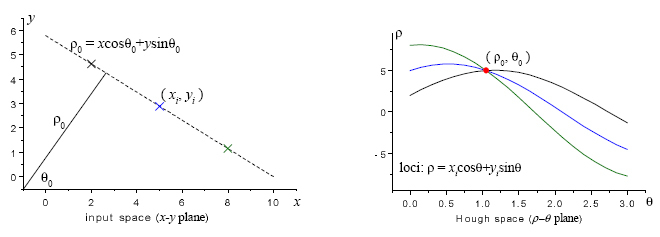
\includegraphics[scale=1]{Pictures/hough_transform.jpeg}
    \caption{Transformata Hougha (źródło:~\cite{Lin:01}).}
    \label{fig:hough_transform}
\end{figure}
\FloatBarrier

Innym spotykanym podejściem~\cite{4410602} jest stosowanie dwóch algorytmów.
Pierwszy z nich ma za zadanie wyodrębnić odcinki linii i pogrupować je na podstawie wcześniej ustalonego zbioru warunków geometrycznych.
Drugi znajduje obszary o najwyższym zagęszczeniu pionowych krawędzi.
Dzięki takiemu spojrzeniu na przedstawiony problem, uzyskane wyniki mają wysoką dokładności, szczególnie dla pojazdów znajdujących się w ruchu.
Metode oparte na krawędziach są stosowane w wielu rozwiązaniach ze względu na ich szybkość działania i prostotę.
Jednakże, rozwiązania te są silenie wrażliwe na niepożądane krawędzie i nie sprawdzają się w rozmytych i złożonych obrazach.

\subsection{Metody oparte na kolorach (ang. \textit{color based)}}
Metody oparte na kolorach bazują na fakcie, że kolor tablicy jest różny od koloru tła pojazdu.
Dla tej grupy rozwiązań, zamiast modelu barw RGB, stosuje się model HSL oparty o nasycenie koloru.
Model ten jest jednak wrażliwy na szum.

Często metody wykorzystujące kolor tablicy rejestracyjnej są używane do wyselekcjonowania kandydatów.
Innymi słowy, oznacza to wybrania obszarów obrazu, w których może znajdować się tablica rejestracyjna.
Technika ta łączona jest z innymi algorytmami, które na kolejnych etapach decydują, czy wskazany obszar rzeczywiście zawiera poszukiwany obiekt.
Do tego typu metod wykorzystywany jest m.\ in.\ algorytm \textit{Mean shift}~\cite{1520110} i logika rozmyta~\cite{Wang2008FuzzybasedAF}.

Opisywana grupa metod może zostać użyta do detekcji zdeformowanych i pochylonych tablic.
Rzadko występują one osobno w metodach detekcji, głównie ze względu na ich dużą czułość na zmiany naświetlenia.
Dodatkowo w zależności od kraju oraz przeznaczenia pojazdu, kolory tablic mogą się znacznie różnić.
Przykładowo obecnie w Polsce tablice aut elektrycznych mają kolor zielony, a samochodów zabytkowych żółty (\ref{fig:tablice}).
\FloatBarrier
\begin{figure}[!ht]
    \centering
    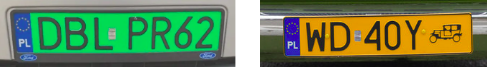
\includegraphics[scale=0.6]{Pictures/tablice}
    \caption{Tablice rejestracyjne w Polsce dla aut elektrycznych i zabytkowych (źródło: opracowanie własne).}
    \label{fig:tablice}
\end{figure}
\FloatBarrier

\subsection{Metody oparte na teksturach (ang. \textit{texture based)}}
\label{subsec:metody-oparte-na-teksturach}
Metody oparte na teksturach wykorzystują fakt znajdowania się znaków na tablicach rejestracyjnych.
Znaki na tablicy mają z reguły czarny kolor i znajdują się na jasnym tle tworząc duży kontrast.
Powyższa grupa algorytmów wykorzystuje wysoką częstość zmiany kolorów w obszarze występowania tablic rejestracyjnych.
W~\cite{824138} autorzy zaproponowali metodę lokalizacji tablic wykorzystując algorytm kwantyzacji wektorów (ang. \textit{Vector Quantization - VQ}).
W przeciwieństwie do innych metod, które wykorzystywały krawędzi lub kontrast, metoda VQ wykorzystuje aktualną zawartość tablicy rejestracyjnej.
Autorzy wykazali bardzo wysoką skuteczność rozwiązania na poziomie 98\%.

W analizie tekstur, często stosuje się filtr Gabora.
Jest to filtr liniowy, pozwalający na przefiltrowanie obrazu z precyzyjnie dobranym zakresem częstotliwości.
Reprezentacje częstotliwości i orientacji filtrów Gabora są uważane przez wielu współczesnych naukowców zajmujących się widzeniem komputerowym za podobne do tych z ludzkiego układu wzrokowego~\cite{gabor_human_eye}.
W~\cite{gabor_lpr} zaprezentowano algorytm wykorzystujący filtr Gabora.
Jest to jednak metoda czasochłonna i nie znajduje zastosowania dla systemów, w których szybkość działania jest jednym z najistotniejszych czynników.

Wszystkie metody oparte na teksturach są odporne na deformacje tablic.
Jest to kluczowa zaleta ich stosowania.
Mimo to, metody te wymagają skomplikowanych obliczeń i nie dają zadowalających efektów w złożonych środowiskach z różnymi warunkami oświetlenia.

\subsection{Klasyfikatory}\label{subsec:klasyfikatory}
Wiele badań wykorzystuje cechy Haara razem ze wzmocnieniem adaptacyjnym (ang. \textit{Adaptative Boosting --- AdaBoost}) do wyuczenia kaskady klasyfikatorów~\cite{9310202}.
Podejście takie zostało zaproponowane po raz pierwszy w~\cite{990517}.
Algorytm Viola-Jones został zaprezentowany w 2001.
Pomimo upływu ponad 20 lat, dalej jest on powszechnie stosowany co świadczy o jego ponadczasowości i uniwersalności.
Autorzy zaprojektowali go jako detektor twarzy, jednak jego funkcjonalność pozwala na wykrywanie dowolnych obiektów, np\. tablic rejestracyjnych, przy odpowiednim wyuczeniu.
Aby przedstawić jak działa algorytm Viola-Jones, należy najpierw zrozumieć czym są cechy Haara.
Cechy Haara często są przedstawiane jako skalowalne, prostokątne szablony (Rysunek~\ref{fig:haar_feats}), używane do porównania zależności pomiędzy pikselami, w szczególności jak ciemne są one względem siebie.
Wartość cechy obliczana jest jako różnica pomiędzy średnią jasnością pikseli w zbiorze ``białym'' i średnią jasnością pikseli w zbiorze ``czarnym''.
\begin{figure}[!ht]
    \centering
    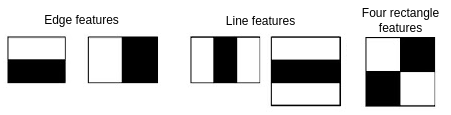
\includegraphics[scale=0.6]{Pictures/haar_feats}
    \caption{Cechy Haara używane w algorytmie Viola-Jones (źródło: \url{https://docs.opencv.org/4.x/d2/d99/tutorial_js_face_detection.html}).}
    \label{fig:haar_feats}
\end{figure}
\FloatBarrier
Podejście takie powoduje jednak, że dla detektora o rozdzielczości 24x24px, algorytm wymaga obliczenia ponad 180000 cech.
Z tego powodu autorzy wprowadzili nowe pojęcie obrazu całkowego (ang. \textit{integral image}).
\begin{theorem}
    Obrazem całkowym nazywamy tablicę dwuwymiarową o rozmiarze obrazu źródłowego, w której każdy element w i-tym wierszu i j-tej kolumnie przechowuje sumę pikseli z tej części obrazu, której prawym dolnym wierzchołkiem jest piksel $(i, j)$ (Rysunek~\ref{fig:ii_cords}).
\end{theorem}
\begin{figure}[!htb]
    \centering
    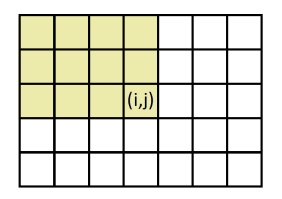
\includegraphics[scale=0.6]{Pictures/ii_cords}
    \caption{Obraz całkowy dla punktu $(i, j)$ (źródło: \url{https://www.spoj.com/WIPING5/problems/WIPING50.pdf}).}
    \label{fig:ii_cords}
\end{figure}
\FloatBarrier
Matematycznie obraz całkowy $ii(x,y)$ przedstawiamy jako:
\begin{equation}
    \label{eq:integral_image}
    ii(x,y) = \sum_{1\leq j \leq x} \sum_{1\leq k \leq y} i(j,k)
\end{equation}
Natomiast obliczanie obrazu całkowego z definicji~\eqref{eq:integral_image} dla każdego punktu w obrazie jest czasochłonne i charakteryzuje się złożonością obliczeniową $O(n_x^2 n_y^2)$.
Aby osiągnąć złożoność niezależną od rozmiaru okna, sumę oblicza się odejmując od sumy wartości obrazu całkowego dla prawego dolnego i lewego górnego wierzchołka sumę wartości obrazu dla pozostałych wierzchołków analizowanego prostokąta.
Poniżej przedstawiono obliczenie sumy dla prostokąta rozpiętego między punktami $(x_1, y_1)$, a $(x_2, y_2)$.
\begin{equation}
    \label{eq:integral_image_x_y}
    \sum_{x_1\leq x \leq x_2} \sum_{y_1\leq y \leq y_2} i(x,y) = ii(x_2, y_2) - ii(x_1 - 1, y_2) - ii(x_2, y_1 - 1) + ii(x_1 - 1, y_1 - 1)
\end{equation}
Na podstawie powyższego wzoru można zauważyć, że wystarczą operacje tylko na 4 punktach obrazu całkowego~\cite{szybka_detekcja_klesk}.
Ten sposób charakteryzuje się liniową złożonością obliczeniową $O(1)$.
Dla obliczenia różnicy pomiędzy sumami dwóch dowolnych prostokątów wymagane jest pobranie wartości dla 8 punktów z obrazu całkowego.

Algorytm Viola-Jones wymaga dużej ilości próbek pozytywnych i negatywnych.
Do wyuczenia klasyfikatora i wybrania zbioru cech zastosowano algorytm AdaBoost.
Autorzy zaproponowali użycie kaskady klasyfikatorów.
Takie podejście bazuje na obserwacji, że okna pozytywne stanowią średnio $0.01\%$ wszystkich okien.
Rozpatrywane okno w pierwszej kolejności badane jest przez słabsze klasyfikatory, które bazują na mniejszej liczbie cech.
Dzięki takiemu podejściu algorytm stał się bardziej wydajny czasowo.
Każdy kolejny klasyfikator w kaskadzie oblicza większą liczbę cech.
Jeżeli na którymś etapie klasyfikator zwróci odpowiedź negatywną, proces jest przerywany.
Do osiągnięcia pozytywnego wyniku, wymagane jest zwrócenie przez wszystkie klasyfikatory odpowiedzi pozytywnej.
W algorytmie Viola-Jones kaskada składa się z 32 klasyfikatorów, które badają od 2 do 200 cech.
Łącznie liczone jest 4297 cech, co daje średnio 8 cech na klasyfikator.
W trakcie uczenia każdy z klasyfikatorów ma przypisany indywidualny próg decyzyjny.
Każdy etap kaskady uczony jest w ramach boostingu (np. poprzez AdaBoost lub
RealBoost).

AdaBoost (Adaptive Boosting) jest popularną techniką wzmacniania, której zadaniem jest stworzenie mocnego klasyfikatora na podstawie wielu słabych klasyfikatorów.
Słabym klasyfikatorem nazywamy klasyfikator, który osiąga niską dokładność, jednak wyższą od losowych wyników.
Za przykład może posłużyć rozpoznawanie płci na podstawie wzrostu.
Słaby klasyfikator mógłby bazować na założeniu, że każda osoba o wzroście 175cm lub wyższym jest mężczyzną.
Pozostała grupa osób jest kobietami.
Wiele osób ze zbioru testowego zostanie określonych błędnie, jednak dokładność klasyfikatora będzie wyższa niż 50\%.

AdaBoost jest techniką, która może zostać łączona z dowolnym algorytmem klasyfikującym, jednak nie może zostać wykorzystany jako samodzielny klasyfikator.
Po raz pierwszy został on przedstawiony w~\cite{Freund1996ExperimentsWA}.
AdaBoost występuję w połączeniu z popularnymi wariantami słabych klasyfikatorów~\cite{szybka_detekcja_klesk}:
\begin{itemize}
    \item AdaBoost + decision stump
    \item AdaBoost + drzewka decyzyjne
    \item AdaBoost + klasyfikator liniowy (np. SVM)
    \item AdaBoost + naiwny Bayes
\end{itemize}
Głównymi zastosowaniami tej techniki jest wybór najlepszych cech z punktu widzenia klasyfikacji oraz dobór wag dla klasyfikatorów wchodzących w skład kaskady.

Każdy słaby klasyfikator powinien zostać wyuczony na losowym podzbiorze zbioru uczącego.
Podzbiory mogą się nakładać, natomiast nie powinno się dzielić zbiorów na równe części.
AdaBoost przypisuje wagi do jednostek treningowych, które określają prawdopodobieństwo pojawienia się w zbiorze uczącym zgodnie ze wzorem~\eqref{eq:treaning_unit_weight_adaboost}.
\begin{equation}
    \label{eq:treaning_unit_weight_adaboost}
    D_{t+1}(i) = \dfrac{D_t(i)exp(-\alpha_t y_i h_t(x_i))}{Z_t}
\end{equation}
$D_t$ oznaczono wektor wszystkich wag, natomiast $Z_t$ reprezentuje ich sumę.
Indeks $i$ jest numerem kolejnej próbki w zbiorze uczącym.
Na początku wszystkie próbki posiadają tą sama wartość wag.
Po zakończeniu uczenia, wagi błędnie sklasyfikowanych próbek zostają zwiększone.
Dzięki temu, w następnej iteracji uczenia kolejny klasyfikator będzie mógł lepiej rozpoznawać niepoprawnie oznaczone jednostki treningowe w poprzednim kroku.
W momencie, gdy każdy klasyfikator zostanie wyuczony, AdaBoost przypisuje do nich wagi na podstawie dokładności każdego z nich.
Ostateczną odpowiedź klasyfikatora można opisać wzorem~\eqref{eq:ada_boost_clf}.
\begin{equation}
    \label{eq:ada_boost_clf}
    H(x) = sign(\sum_{T}^{t=1} \alpha_t h_t(x))
\end{equation}
Finalny klasyfikator zawiera $T$ słabych klasyfikatorów.
Waga klasyfikatora, wyliczona przez AdaBoost, została określona symbolem $\alpha_t$.
Ostateczny rezultat powyższego równania można opisać jako liniowa kombinacja słabych klasyfikatorów.

Pierwszy klasyfikator ($t=1$) jest trenowany z równym prawdopodobieństwem dla wszystkich próbek.
Po zakończeniu uczenia, waga obliczana jest na podstawie wzoru~\eqref{eq:weight_clf}.
\begin{equation}
    \label{eq:weight_clf}
    \alpha_t = \dfrac{1}{2} \ln \dfrac{1-\epsilon_t}{\epsilon_t}
\end{equation}
Współczynnik $\alpha_t$ jest skorelowany z poziomem błędu klasyfikatora $\epsilon_t$, który to jest liczony jako liczba błędnie sklasyfikowanych próbek dzielona przez rozmiar zbioru uczącego.
Rysunek~\ref{fig:adaboost_alphacurve} przedstawia powyższą zależność.
\begin{figure}[!ht]
    \centering
    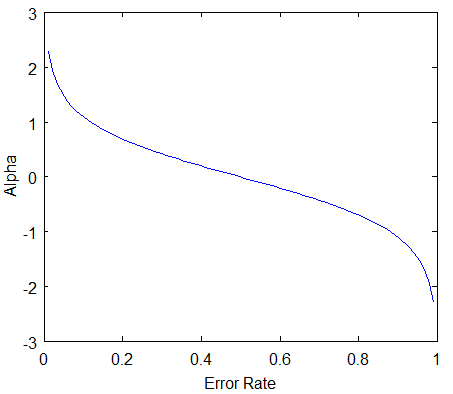
\includegraphics[scale=0.6]{Pictures/adaboost_alphacurve}
    \caption{Zależność współczynnika $\alpha$ od błędu klasyfikatora (źródło: \url{https://chrisjmccormick.files.wordpress.com/2013/12/adaboost_alphacurve.png}).}
    \label{fig:adaboost_alphacurve}
\end{figure}
\FloatBarrier
Z Rysunku~\ref{fig:adaboost_alphacurve} można odczytać, że waga rośnie wykładniczo dla klasyfikatorów o wysokiej dokładności.
Dla klasyfikatora o poziomie błędu 0.5 waga jest równa zero.
Oznacza to, że taki klasyfikator jest równie dokładny co losowe zgadywanie, dlatego jest on ignorowany.
Dla klasyfikatorów o większym poziomie błędu, waga przyjmuje wartość ujemną.
Jeśli taki klasyfikator uzna próbkę za negatywną, ostatecznie zostanie ona oznaczona jako pozytywna.

AdaBoost jest techniką uczenia progresywnego.
Ważne jest, aby na wejściu próbki uczące były odpowiedniej jakości.
Metoda ta jest bardzo czuła na zakłócenia.
Jednymi z najczęstszych aplikacji tego typu boostingu jest klasyfikacja tekstu oraz zdjęć.

Wzmocnienie AdaBoost spotykane jest w różnych wariantach.
Jednym z nich jest Real AdaBoost, zwany również RealBoostem, zaprezentowany po raz pierwszy w~\cite{10.1023/A:1007614523901}.
Główną różnicą w stosunku do AdaBoosta, jest założenie, że słabe klasyfikatory są rzeczywistoliczbowe, a nie binarne~\cite{szybka_detekcja_klesk}.
Odpowiedź słabego klasyfikatora jest zwykle ustalana jako przybliżenie połowy przekształcenia logit:
\begin{equation}
    \label{eq:real_boost}
    f_t(X) =\dfrac{1}{2}\ln\dfrac{\hat{P_w}(y=1|x)}{\hat{P_w}(y=-1|x)}
\end{equation}
gdzie $\hat{P_w}(y=\pm1|x)$ stanowi oszacowanie rozkładu klas warunkowego na $x$ z wykorzystaniem aktualnych wag $w_i$.
W przeciwieństwie do AdaBoost, słabe klasyfikatory nie posiadają wag.
Mechanizm ważenia słabych klasyfikator jest niejako wpleciony w same odpowiedzi rzeczywistoliczbowe.
Możliwym jest wykazanie, że wyrażenie~\eqref{eq:real_boost} jest rozwiązaniem zadania minimalizacji kryterium wykładniczego określonego poprzez rozkład ${w_i}$ na zbiorze danych (tj.\ na konkretnej próbie).
Analogicznie wyrażenie to jest również rozwiązaniem zadania minimalizacji kryterium wykładniczego określonego poprzez prawdziwy ale nieznany rozkład łączny generujący dane tj. $P(x,y)=p(x)P(y|x)$~\cite{szybka_detekcja_klesk}.
Algorytm RealBoost posiada silne podobieństwa do techniki regresji logistycznej.
Schemat reważenia w boostingu pracuje sposób pokrewny do rezyduów błędów (ang. \textit{error residuals}).

%TODO - poprawka koszyków
Jednym ze słabych klasyfikatorów stosowanych razem z algorytmem RealBoost są tzw.\ koszyki (ang. \textit{response binning}).
Ten typ klasyfikatora został zaprezentowany w~\cite{1689652}.
Przedstawiony sposób działania polega na przybliżaniu rozkładów warunkowych przez funkcje kawałkami stałe~\cite{szybka_detekcja_klesk}.
Przed uczeniem algorytmu wyznacza na jest liczba koszyków o równej szerokości oznaczana literą $B$.
Na podstawie ustalonych przedziałów $[a_1,a_2]$, każdej z cech przypisywany jest odpowiedni indeks koszyka.
Indeks koszyka $\beta(x) \in \{1,\dots,B\}$, do którego należy $x$ obliczany jest na podstawie wzoru~\eqref{eq:bin_index}.
\begin{equation}
    \label{eq:bin_index}
    \beta(x)=\left.
    \begin{cases}
        B(x - a_1)/(a_2-a_1), & \text{dla } a_1 \leq x \leq a_2 \\
        1, & \text{dla } x \leq a_1 \\
        B, & \text{dla } a_2 < x
    \end{cases}
    \right.
\end{equation}
Odpowiedź słabego klasyfikatora dla $j^*$-tej cechy przedstawia wzór~\eqref{eq:bin_weak_clf}, gdzie $\hat{P_w}(y=-1, j\;jest\;w\;b)=\sum_{\{i:y_i=-1,\beta(x_ij)=b\}}^{} w_i$ oznacza szacowane prawdopodobieństwo zdarzenia, że przykład jest negatywny a jego $j$-ta cecha należy do kosza $b$.
\begin{equation}
    \label{eq:bin_weak_clf}
    f_t(x;j^*) = \dfrac{1}{2} \ln\dfrac{\hat{P_w}(y=1, j^*\;jest\;w\;\beta(x_j^*))}{\hat{P_w}(y=-1, j^*\;jest\;w\;\beta(x_j^*))}
\end{equation}
Autorzy algorytmu zalecają stosowanie dużej ilości koszyków dla gładkiego histogramu rozkładu cech.
Jeżeli histogram zawiera wiele maksimum lokalnych, należy zmniejszyć ilość koszyków.
W przeciwnym razie zbyt duża rozdzielczość może wprowadzić szum do klasyfikatora, natomiast zbyt niska liczba koszyków może pozbawić klasyfikatora istotnych cech~\cite{1689652}.

\subsection{Metody głębokiego uczenia (ang. \textit{Deep learning})}
W związku z rozwojem dziedziny widzenia komputerowego oraz wzrostem mocy komputerów na przestrzeni ostatnich lat, wiele metod statystycznych zostało zastąpionych przez sieci neuronowe z powodu ich wysokiej skuteczności w detekcji obiektów.
Jednym z zaproponowanych podejść jest użycie sieci konwolucyjnych (ang. \textit{Convolutional Neural Network} --- CNN)\cite{cnn_detector}.
Składają się one z jednej lub wielu warstw konwolucyjnych (typowych dla kroku próbkowania, określającego subwzorce), a następnie przez jedną lub w pełni połączone warstwy tak jak w klasycznej wielowarstwowej sieci, np. MLP,SVM, SoftMax itp.
Sieci kowolucyjne są łatwe do uczenia, gdyż zawierają mniej parametrów (wykorzystując te same wagi) niż typowe sieci neuronowe z dokładnością do ilości warstw konwolucyjnych i ich rozmiaru.
Ten rodzaj sieci neuronowych jest predestynowany do obliczeń na strukturach 2D (tj\. obrazy)~\cite{cnn_agh}.

Jednym z najnowocześniejszych systemów detekcji w czasie rzeczywistych jest algorytm YOLO (ang. \textit{You only look once})~\cite{7780460}.
Algorytm jest bardzo wydajny.
Bazuje na sieciach R-CNN.
Autorzy zapewniają o możliwości przetwarzania 45 klatek na sekundę, a dla wersji szybszej, lecz o niższej dokładności, ponad 150 klatek na sekundę.
Twórcom wzorca przyświecała idea ``spojrzenia tylko raz'', wzorując się na postrzeganiu świata przez człowieka, który po jednym spojrzeniu na badany obraz, jest w stanie zidentyfikować konkretne obiekty.
W przeciwieństwie do tradycyjnych metod z oknem przesuwnym, YOLO podczas procesu uczenia i testowania otrzymuje na wejściu cały obraz.
Na obraz wejściowy nałożona zostaje siatka o rozmiarze SxS, która tworzy obwiednie, a następnie wykorzystuje je do rozpoznawania szukanych obiektów.
Dla każdej uzyskanej ramki, mechanizm wyznacza prawdopodobną klasę.
Ramki o prawdopodobieństwie wyższym od ustalonego progu, zostają nałożone na wejściowy obraz, najczęściej w postaci prostokątów otaczających obiekt.
Rysunek~\ref{fig:yolo} przedstawia opisany schemat.
Ograniczenia YOLO wynikają z ograniczeń przestrzennych algorytmu.
W zależności od wielkości siatki, system może mieć problem z wykryciem mniejszych obiektów takich jak np. stado ptaków.
Algorytm jest stale udoskonalany przez autorów.
Na moment pisania pracy, udostępniona została trzecia wersja systemu.
\begin{figure}[!ht]
    \centering
    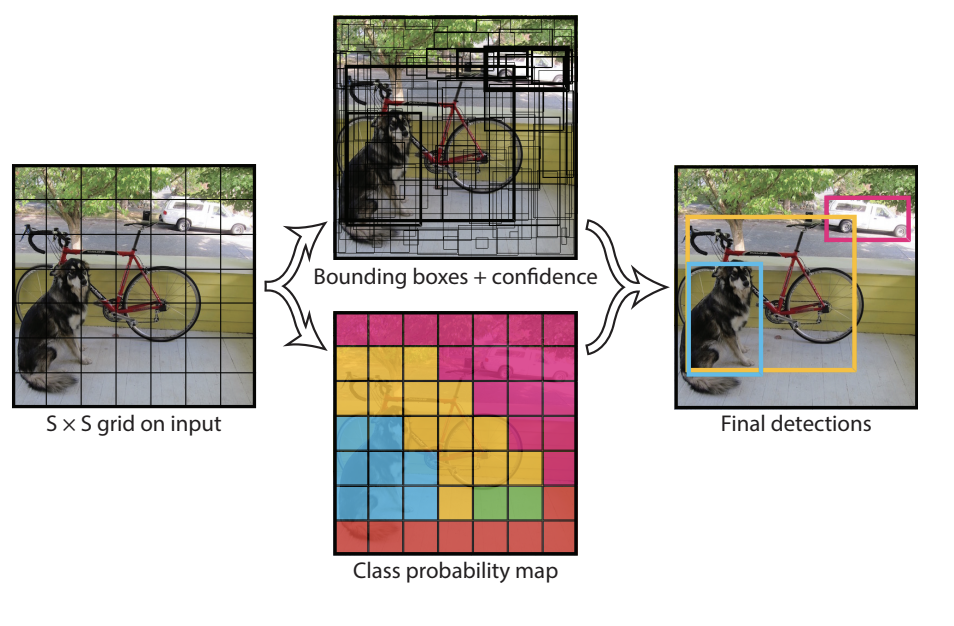
\includegraphics[scale=0.4]{Pictures/yolo}
    \caption{Algorytm YOLO (źródło: \url{https://towardsdatascience.com/r-cnn-fast-r-cnn-faster-r-cnn-yolo-object-detection-algorithms-36d53571365e}).}
    \label{fig:yolo}
\end{figure}
\FloatBarrier


\section{Przegląd istniejących metod segmentacji tablic rejestracyjnych}
\index{Przegląd istniejących metod segmentacji tablic rejestracyjnych}

Drugim etapem w większości systemów Automatycznego Rozpoznawania Tablic Rejestracyjnych jest rozpoznanie znaków na tablicy rejestracyjnej zlokalizowanej w poprzednim kroku.
Zanim dojdzie do klasyfikacji znaków, często są one wpierw segmentowane.
Jest to szczególny przypadek optycznego rozpoznawania znaków~\cite{9310202}.
Wiele krajów posiada ścisłe regulacje na temat czcionki i kolorów tablicy rejestracyjnej.
Przepisy te mają na celu zwiększenie czytelności znaków identyfikujących każdy pojazd.
W Polsce, jak i większości krajów na świecie, tablice pokryte są specjalną warstwą refleksyjną odbijającą światło.
Działanie takie zwiększa ich czytelność dla ludzkiego oka w gorszych warunkach oświetleniowych.
Dla aparatów fotograficznych ta cecha tablic często powoduje nieczytelność tablic na wykonanym zdjęciu.
Tablica odbija na tyle dużą ilość światła, co skutkuje powstaniem na zdjęciu białego prostokąta w miejscu tablicy.
Przykład takiego obrazu przedstawia Rysunek~\ref{fig:refleks_swietlny}.
\begin{figure}[!ht]
    \centering
    \includegraphics[scale=0.8]{Pictures/refleks_świetlny}
    \caption{Refleks świetlny występujący w niewystarczających warunkach oświetleniowych (źródło: opracowanie własne).}
    \label{fig:refleks_swietlny}
\end{figure}
\FloatBarrier
Poza powyższymi trudnościami, tablice mogą być obrócone lub uszkodzone.
Aby zwiększyć w jak największym stopniu prawdopodobieństwo prawidłowego odczytania znaków, używa się szereg czynności na obrazie wejściowym.
Dla obróconych obiektów stosuje się transformatę biliniową, zwaną również metodą Tustina~\cite{Xu2006AMO}.

\subsection{Binaryzacja}\label{subsec:binaryzacja}
W wielu klasycznych metodach widzenia komputerowego, w celu segmentacji znaków, stosuje się binaryzację.
W zbinaryzowanym obrazie łatwiej jest rozdzielić znaki w porównaniu do obrazu kolorowego lub w skali szarości.
Podstawowym problemem tej techniki jest odpowiedni dobór wartości progu.
Wybór ten jest dokonywany w oparciu o różne metody, które można podzielić na zmiennoprogowe i automatyczne.
Jednakże, wyznaczenie progu binaryzacji musi zostać wykonane właściwie, w celu uniknięcia połączenia znaków lub scalenia ich z obramowaniem tablicy rejestracyjnej~\cite{6213519}.
Jednym z częściej stosowanych metod binaryzacji jest progowanie adaptacyjne (ang. \textit{Adaptive Thresholding}).
Stosuje się to w momencie kiedy różne obszary obrazu mogą charakteryzować się różnymi warunkami oświetlenia i stosowanie stałej wartości nie dałoby zadowalających efektów.
Algorytm wyznacza próg dla konkretnego piksela na podstawie niewielkiego regionu wokoło.
Dla tego samego obrazu wyliczane są różne wartości progu dla różnych regionów co prowadzi do uzyskania lepszych wyników niż w przypadku stałego progu binaryzacji.
Na Rysunku~\ref{fig:threshold} przedstawiono przykłady binaryzacji obrazu stałym progiem globalnym i progiem wyznaczonym adaptacyjnie.
\begin{figure}[!ht]
    \centering
    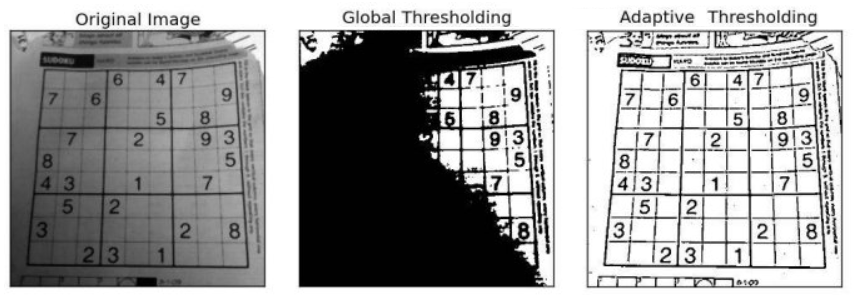
\includegraphics[scale=0.6]{Pictures/threshold}
    \caption{Przykład binaryzacji obrazu przy niejednorodnym oświetleniu za pomocą globalnego i lokalnego progu (źródło: \url{https://docs.opencv.org/3.4/d7/d4d/tutorial_py_thresholding.html}).}
    \label{fig:threshold}
\end{figure}
\FloatBarrier

Algorytm progowania adaptacyjnego otrzymuje najczęściej na wejściu obraz w skali szarości lub kolorowy.
Próg jest wyliczany dla wszystkich pikseli w obrazie z osobna.
Jednym ze znanych podejść jest to zaproponowane przez Chow i Kaneko~\cite{Chow1971BoundaryDO}.
W tym przypadku obraz dzielony jest na zbiór nakładających się fragmentów.
Optymalny próg wyznaczy jest dla konkretnego fragmentu na podstawie analizy histogramu.
Próg dla każdego piksela wyliczany jest na podstawie interpolacji wyników dla odpowiedniego fragmentu.
Wadą tej metody jest jej złożoność obliczeniowa.
Jest to jeden z głównych powodów, dlaczego algorytm ten nie znalazł zastosowania w aplikacjach działających w czasie rzeczywistym.

Alternatywnym podejściem do znalezienia lokalnego progu jest statystyczne zbadanie intensywności sąsiedztwa każdego piksela.
Wybór metody statystycznej jest skorelowany z obrazem wejściowym.
Najczęściej używa się średniej, mediany, średniej z wartości maksymalnej i minimalnej badanego otoczenia lub funkcji Gaussa.
Dobór wielkości sąsiedztwa ma duży wpływ na wyliczenie progu.
Rozmiar musi być na tyle duży, aby zawierać zarówno piksele tła jak i badanego obiektu.
Z drugiej strony wybranie zbyt dużych obszarów może naruszyć założenie o równomiernym oświetleniu rozpatrywanego fragmentu.
Ten rodzaj adaptycyjnego progowania jest bardziej wydajny od algorytmu Chow i Kaneko.
Charakteryzuje się wysoką jakością oddzielania obiektów od tła i znajduje szerokie zastosowanie w wielu aplikacjach.

Innym znanym algorytmem stosowanym do wyznaczania progu binaryzacji jest algorytm Otsu~\cite{4310076}.
Metoda Otsu jest techniką opartą na wariancji w celu znalezienia wartości progowej, przy której ważona wariancja między pikselami pierwszego planu i tła jest najmniejsza~\cite{otsu_article}.
Kluczową ideą jest tutaj iteracja przez wszystkie możliwe wartości progu i pomiar rozproszenia pikseli tła i pierwszego planu.
Następnie znajdowany jest próg, w którym rozproszenie jest najmniejsze.
Algorytm iteracyjnie wyszukuje próg, który minimalizuje wariancję wewnątrz klasy, zdefiniowaną jako ważona suma wariancji dwóch klas (tła i pierwszego planu).
Kolory w skali szarości zwykle mieszczą się w zakresie 0-255.
Tak więc, jeśli wybierzemy próg 100, to wszystkie piksele o wartościach mniejszych niż 100 staną się tłem, a wszystkie piksele o wartościach większych lub równych 100 staną się pierwszym planem obrazu.
Wzór na znalezienie wariancji wewnątrz klasowej przy dowolnym progu $t$ jest określony wzorem~\eqref{eq:otsu_variance}
\begin{equation}
    \label{eq:otsu_variance}
    \sigma^2(t)=\omega_{bg}(t)\sigma_{bg}^2(t)+\omega_{fg}(t)\sigma_{fg}^2(t)
\end{equation}
gdzie $\omega_{bg}(t)$ i $\omega_{fg}(t)$ reprezentują prawdopodobieństwo liczby pikseli dla każdej klasy przy progu $t$, natomiast $\sigma^2$ oznaczono wariancję wartości kolorów.
Wyliczanie wariancji dla konkretnej klasy pikseli przedstawiono na wzorze~\eqref{eq:otsu_variance_value}.
\begin{equation}
    \label{eq:otsu_variance_value}
    \sigma_{bg | fg}^2(t)=\dfrac{\sum_{}^{}(x_i-\hat{x})^2}{N-1}
\end{equation}
Wartość piksela odpowiedniej klasy reprezentuje symbol $x_i$, natomiast $\hat{x}$ reprezentuje średnią pikseli rozpatrywanej klasy.
Liczbę wszystkich pikseli zapisano literą $N$.

Metoda Otsu implementowana przez wiele środowisk obliczeniowych (np. MATLAB)~\cite{otsu_inzynieria_rolnicza}.
Algorytm szczególnie dobrze sprawdza się w przypadkach, gdy liczby pikseli tła i obiektów pierwszego planu są zbliżone~\cite{10.1117/1.1631315}.

\subsection{Metoda k-średnich (ang. \textit{ang. K-Means algorithm})}
todo~\cite{segmentation_kmeans}

\subsection{Metoda rzutów jasności}
todo

\subsection{Metoda elementów połączonych (ang. \textit{Connected components})}
todo


\section{Przegląd istniejących metod rozpoznawania tablic rejestracyjnych}
\index{Przegląd istniejących metod rozpoznawania tablic rejestracyjnych}

\subsection{OCR}
tesseract korzysta z sieci lstm wiec warto by to opisać i jakieś inne sieci
%https://bulldogjob.pl/readme/3-typy-rekurencyjnych-sieci-neuronowych

\subsection{Metody oparte na wzorcach}
@TODO - TEMPLATE AND PATTERN MATCHING TECHNIQUES